\newcommand{\TeamNo}{31}

\newcommand{\HWno}{02}

\newcommand{\AuthorOneName}{Merve Nur Öztürk}
\newcommand{\AuthorOneID}{2311322}

\newcommand{\AuthorTwoName}{Atakan Süslü}
\newcommand{\AuthorTwoID}{2311371}

\newcommand{\AuthorThreeName}{Betül Rana Kuran}
\newcommand{\AuthorThreeID}{2311173}


\documentclass[letterpaper,12pt]{article}
\usepackage{tabularx} % extra features for tabular environment
\usepackage{amsmath}  % improve math presentation
\usepackage{amssymb}
\usepackage{xcolor}
\usepackage{float}
\usepackage[export]{adjustbox}
\usepackage{graphicx} % takes care of graphic including machinery
\usepackage[margin=1in,letterpaper]{geometry} % decreases margins
\usepackage{cite} % takes care of citations

\begin{document}
\begin{center}
AE 305, 2020-21 Fall \hfill \textbf{HW \HWno} \hfill \textbf{Team \TeamNo} \\
\noindent\rule{\textwidth}{0.4pt}
\begin{tabular}{p{0.33\textwidth} | p{0.33\textwidth} | p{0.33\textwidth} }
	\AuthorOneName&\AuthorTwoName&\AuthorThreeName\\
	\textit{\AuthorOneID}&\textit{\AuthorTwoID}&\textit{\AuthorThreeID}
\end{tabular}
\noindent\rule{\textwidth}{0.4pt}
\end{center}

%Report start

\section{Introduction}

Numerical methods, such as Runge Kutta Method, are widely used to solve differential equations when an
analytical solution is not possible or time-consuming. $4^{th}$ order Runge-Kutta Method is one of the
numerical methods which gives quite accurate results due to its small truncation error. In this homework,
a solid propellent rocket is given, and its chamber pressure $p_c$, burn rate $\dot{r}$, and the specific
impulse $I_{sp}$ are asked to be calculated with this method until the chamber pressure $p_c$ becomes equal 
to the atmospheric pressure $p_a$, with different time step sizes and different nozzle throat radiuses.

This equation gives the rate of the chamber pressure of the given rocket with a constant burn temperature
$T_c$:

\begin{equation}
	\frac{dp_c}{dt} = \frac{RT_c}{V_c}(\dot{m_{bs}} - \dot{m_{ce}} - \rho_{c}\dot{V_c})
\end{equation}

It is assumed that the propellant inner surface is circular and between the chamber exit and nozzle throat
no gas mass accumulates ($\dot{m_{ce}} = \dot{m_n}$). Moreover, writing $\dot{m_{bs}} = \rho_{p}2\pi rL\dot{r}$,
and $V_c = \pi r^{2}L$, the equation becomes:

\begin{equation}
	\frac{dp_c}{dt} = RT_c[\frac{2\dot{r}}{r}(\rho_{p} - \rho_{c}) - \frac{\dot{m_n}}{\pi r^{2}L}]
\end{equation}

It is given that $\dot{r} = ap_c^{n}$, and $\dot{m_n} = p_cA^{*}\sqrt{\frac{\gamma}{RT_c}}(\frac{\gamma +1}{2})^{-\frac{\gamma +1}{2(\gamma -1)}}$
where $A^{*}$ is the nozzle throat area. Furthermore, though at first it was assumed that the propellant 
inner surface is circular, it is more of a complex shape. Thus, a propellant design dependent factor
$f_{cor}(r)$ is used to simply approach to original characteristics. Then, the equations for the rate
of chamber pressure, and the rate of equivalent radius r become:

\begin{equation}
	\boxed{\frac{dp_c}{dt} = RT_c[f_{cor}(r)\frac{2ap_c^{n}}{r}(\rho_{p} - \frac{p_c}{RT_c}) - \frac{p_cA^{*}}{\pi r^{2}L}\sqrt{\frac{\gamma}{RT_c}}(\frac{\gamma +1}{2})^{-\frac{\gamma +1}{2(\gamma -1)}}]}
\end{equation}

\begin{equation}
	\boxed{\frac{dr}{dt} = ap_c^{n}}
\end{equation}

Specific impulse is also asked to be calculated, and its formula is:

\begin{equation}
	\boxed{I_{sp} = \frac{1}{g}\sqrt{\frac{2\gamma RT_c}{\gamma -1}[1-(\frac{p_a}{p_c})^{\frac{\gamma -1}{\gamma}}]}}
\end{equation}

\section{Method}

\newpage

\section{Results and Discussion}

% Görmek için koydum, yazarken silin
\begin{figure}
	\centering
	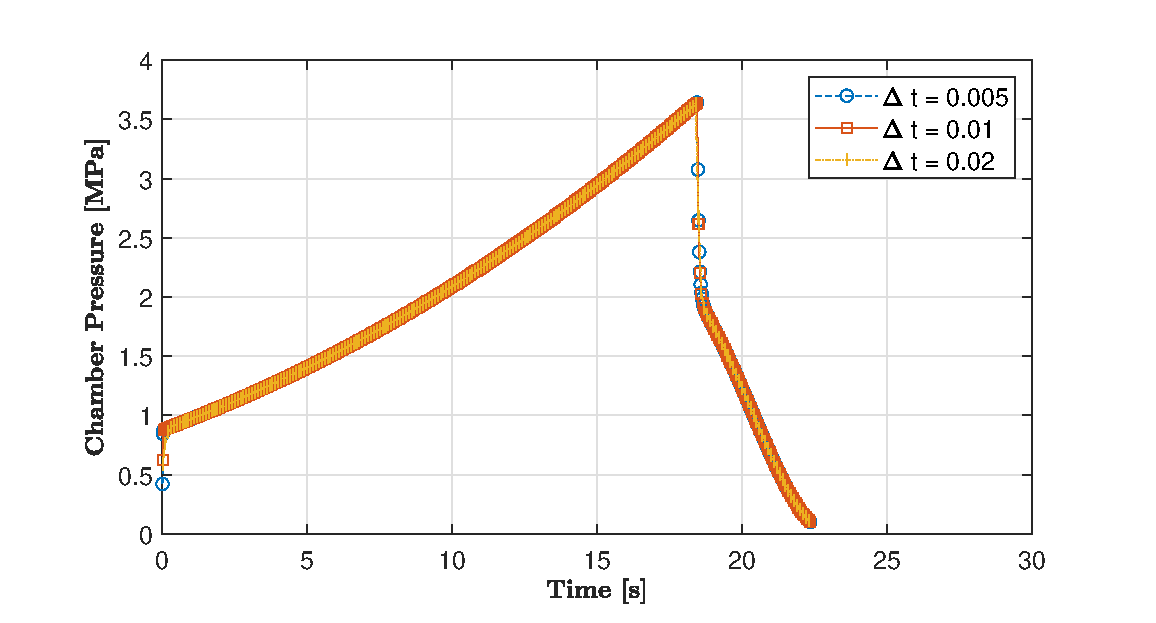
\includegraphics[height = 8.5cm]{graphs/q1_pc.eps}
\end{figure}
\begin{figure}
	\centering
	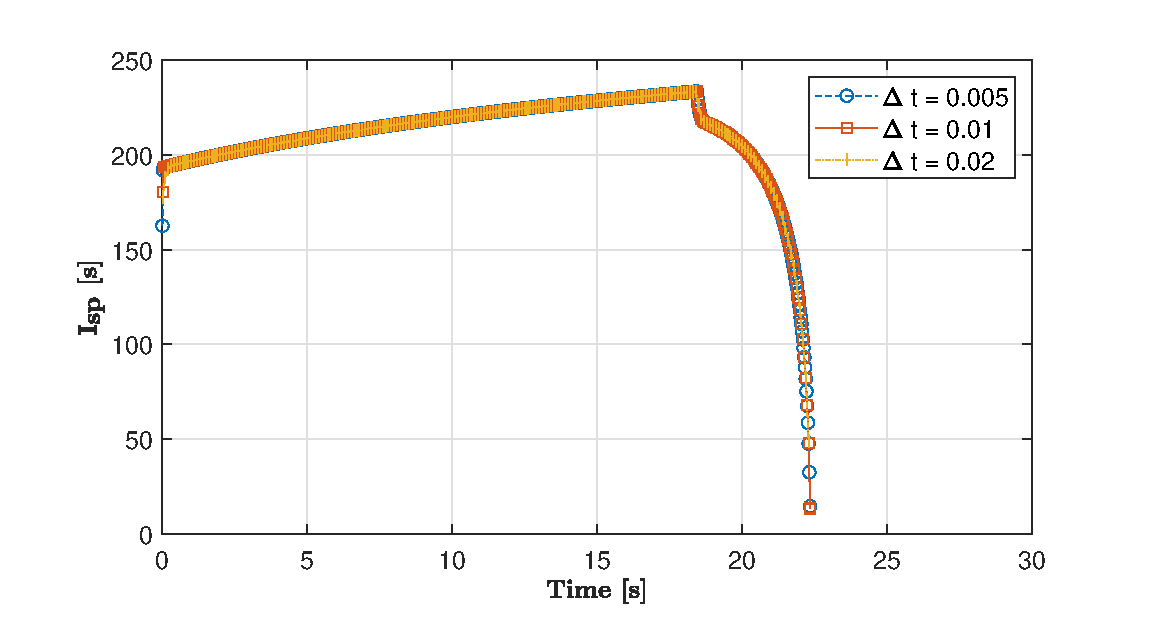
\includegraphics[height = 8.5cm]{graphs/q1_isp.eps}
\end{figure}
\begin{figure}
	\centering
	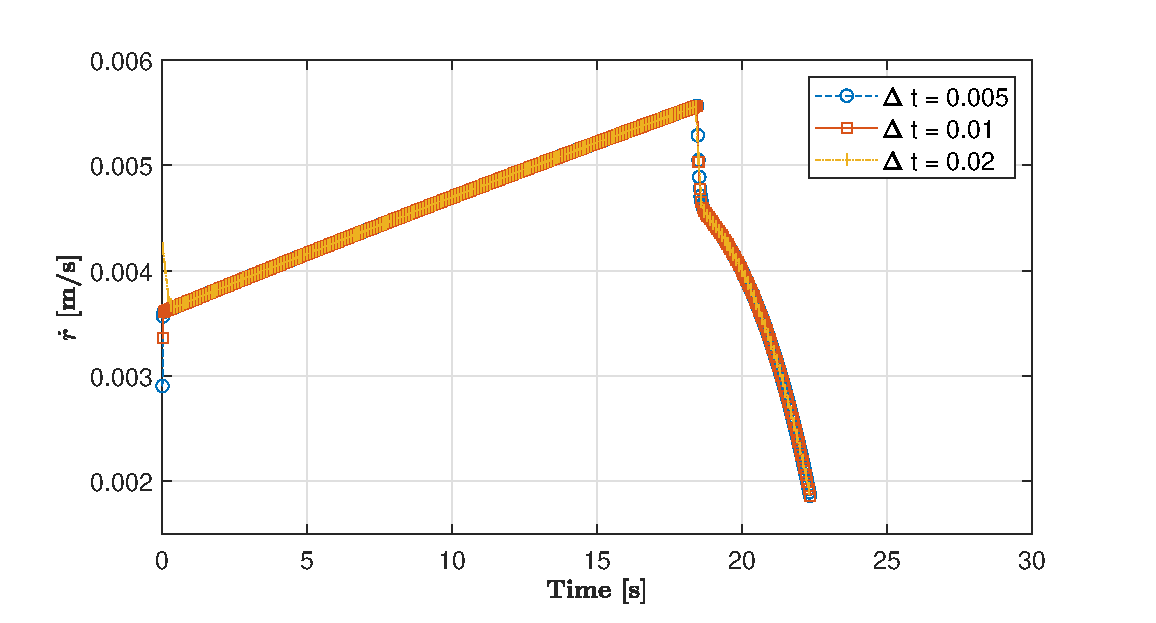
\includegraphics[height = 8.5cm]{graphs/q1_rdot.eps}
\end{figure}
\begin{figure}
	\centering
	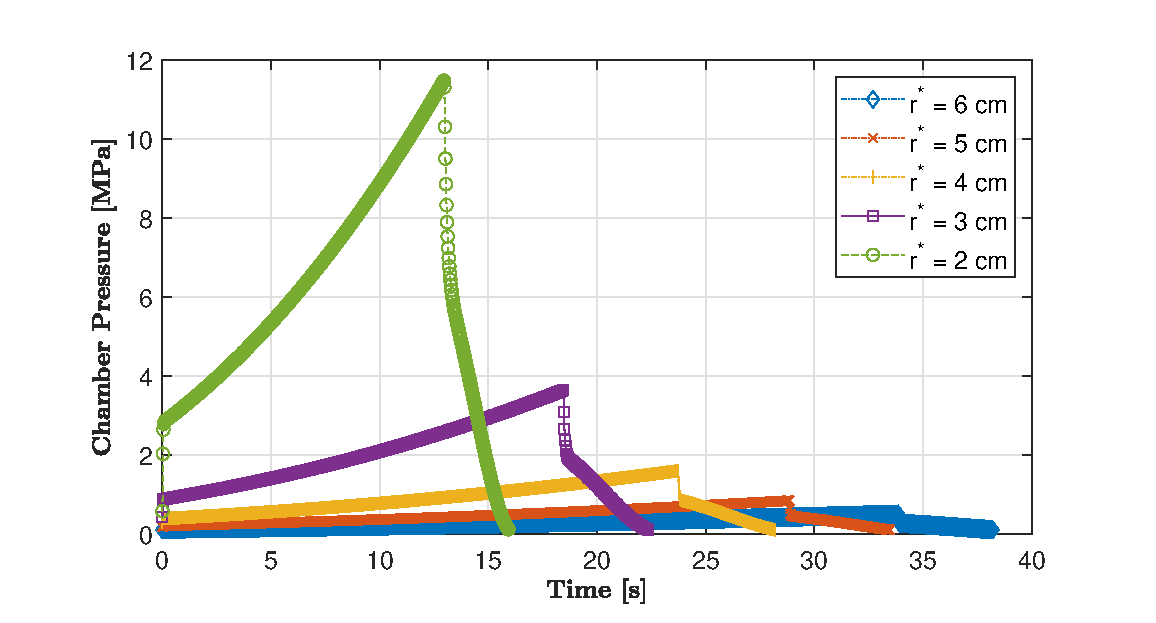
\includegraphics[height = 8.5cm]{graphs/q2_pc.eps}
\end{figure}
\begin{figure}
	\centering
	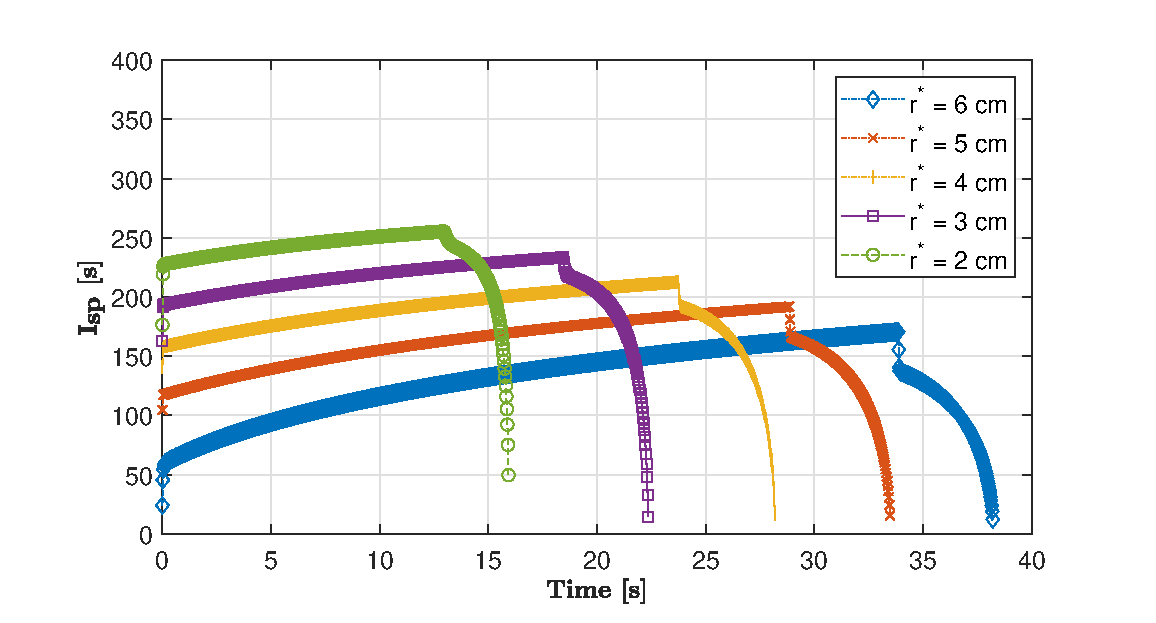
\includegraphics[height = 8.5cm]{graphs/q2_isp.eps}
\end{figure}
\begin{figure}
	\centering
	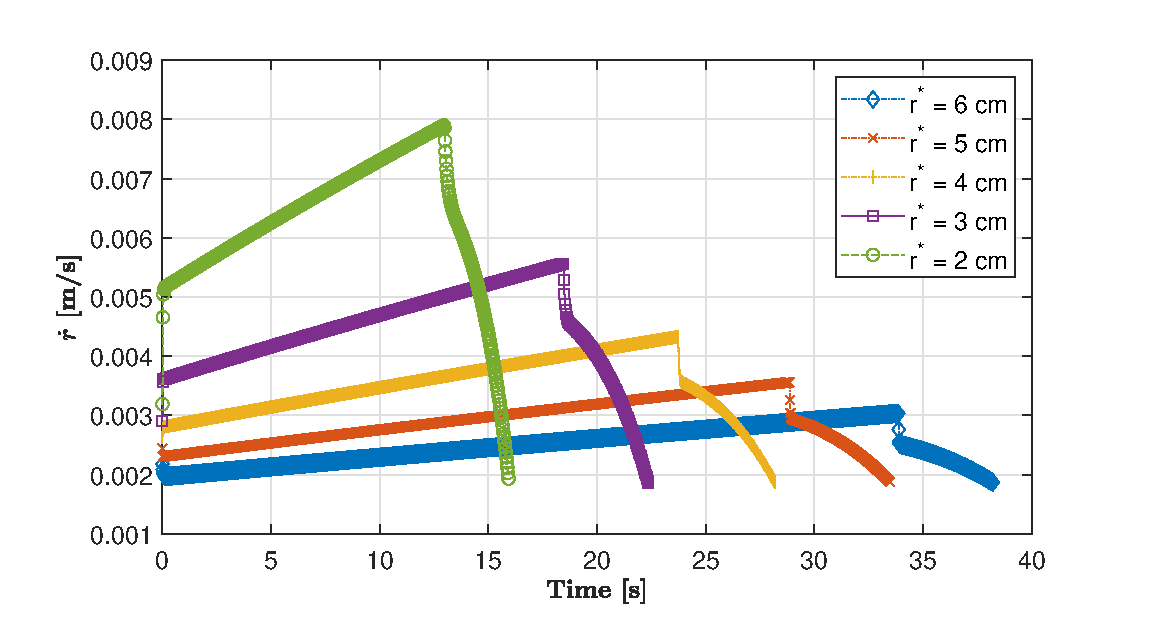
\includegraphics[height = 8.5cm]{graphs/q2_rdot.eps}
\end{figure}
\section{Conclusion}

\end{document}